% ============================================================================
% CHAPITRE 6 — TESTS, ÉVALUATION ET RÉSULTATS
% ============================================================================

\section{Introduction}

Ce chapitre évalue les deux sous-systèmes de Guidni à travers des approches complémentaires~:
tests unitaires pour la correction mathématique, tests d'intégration pour les cycles de vie
complets des requêtes, et évaluation empirique des performances de l'intelligence artificielle.
L'évaluation couvre quatre dimensions~: la qualité de l'agent planificateur, la précision du
pipeline RAG, la performance d'apprentissage du moteur de recommandation, et les performances
globales du système.

La méthodologie combine des vérifications automatisées (blocs \texttt{\_\_main\_\_} intégrés
dans chaque module, exécutables par \texttt{python -m app.reco.context}) avec des sessions
d'évaluation manuelle sur des scénarios réalistes. Les résultats sont présentés avec des
métriques quantitatives (latence, précision, récompense cumulée) et des analyses qualitatives
(cohérence des plans, pertinence des recommandations).


% ────────────────────────────────────────────────────────────────
\section{Stratégie de test}
% ────────────────────────────────────────────────────────────────

L'évaluation d'un système d'intelligence artificielle requiert plus que la simple vérification
de son exécution   elle nécessite la validation de la correction mathématique au niveau des
composants, la justesse fonctionnelle au niveau de l'intégration, et la qualité comportementale
au niveau des scénarios. Chaque niveau capture une classe distincte de défauts qui échapperait
aux autres. Cette stratégie à trois niveaux a été choisie car les deux sous-systèmes
présentent des modes de défaillance fondamentalement différents (erreurs mathématiques
pour le LinUCB contre erreurs de raisonnement pour l'agent LLM).

La pyramide de tests adoptée comprend trois niveaux, comme le résume le tableau~\ref{tab:test_coverage}. Les tests unitaires vérifient la
correction mathématique des composants individuels~: le module d'ingénierie des caractéristiques (forme du vecteur
$\phi$, résilience aux NaN/inf, encodage cyclique), le moteur de scoring LinUCB (scoring UCB,
règle de mise à jour, calcul de récompenses, santé matricielle), et le pipeline de classement
(chaque étape du pipeline de classement). Les tests d'intégration vérifient les cycles
complets~: aller-retour via les endpoints de planification conversationnelle avec génération de plan, boucle de validation avec
correction d'erreurs, traitement par lots d'événements avec mise à jour des matrices. Les
évaluations manuelles de bout en bout simulent des scénarios utilisateur réalistes avec
différents fournisseurs LLM et différentes langues.

L'environnement de test utilise une base de données PostgreSQL alimentée avec les annonces
réelles de Djerba (activités, hébergements, restaurants), Ollama exécutant un modèle
open-source local pour les tests hors ligne, et un index RAG LlamaIndex construit à partir des mêmes
données de référence. Les fournisseurs cloud (Groq, Gemini) sont testés en complément pour
valider la compatibilité multi-fournisseurs.

Ces blocs d'auto-test constituent la première ligne de défense, vérifiant la correction
mathématique des calculs de vecteurs, de scoring et de récompenses sur des cas limites
connus avant tout déploiement.

\begin{table}[H]
    \centering
    \caption{Matrice de couverture des tests}
    \label{tab:test_coverage}
    \footnotesize
    \begin{tabular}{p{4.5cm} c c c}
        \toprule
        \textbf{Composant} & \textbf{Unitaire} & \textbf{Intégration} & \textbf{Manuel} \\
        \midrule
        Construction du vecteur utilisateur & \checkmark & — & — \\
        Construction du vecteur phi & \checkmark & — & — \\
        Correspondance budgétaire & \checkmark & — & — \\
        Calcul du score UCB & \checkmark & — & — \\
        Mise à jour des matrices & \checkmark & — & — \\
        Calcul de récompense delta & \checkmark & — & — \\
        Santé matricielle & \checkmark & — & — \\
        Réinitialisation partielle & \checkmark & — & — \\
        Pipeline de classement (10 étapes) & \checkmark & — & — \\
        POST /chat & — & \checkmark & \checkmark \\
        POST /plan & — & \checkmark & \checkmark \\
        GET /api/recommendations & — & \checkmark & \checkmark \\
        POST /events (batch) & — & \checkmark & — \\
        RAG indexation & — & \checkmark & — \\
        RAG requête & — & \checkmark & \checkmark \\
        Mémoire / résumé & — & \checkmark & \checkmark \\
        Fournisseur LLM factory & — & \checkmark & — \\
        \bottomrule
    \end{tabular}
\end{table}


% ────────────────────────────────────────────────────────────────
\section{Évaluation de l'agent planificateur}
% ────────────────────────────────────────────────────────────────

\subsection{Scénarios de test}

Six scénarios de test ont été définis pour couvrir les cas d'usage principaux de l'agent
planificateur. Chaque scénario spécifie un contexte utilisateur (type de voyage, durée,
budget), des contraintes spécifiques, le fournisseur LLM utilisé, et le résultat attendu.
Les scénarios couvrent la gamme complète des fonctionnalités~: génération simple, planification
longue, modification de plan existant, multilinguisme, et gestion des requêtes incomplètes, comme le montre le tableau~\ref{tab:test_scenarios}.

Les scénarios SC-04 et SC-05 testent spécifiquement la capacité multilingue de l'agent~:
le prompt système instruite l'agent de détecter automatiquement la langue de l'utilisateur et
de répondre dans la même langue. Le scénario SC-06 teste le déclenchement de l'outil
\texttt{ask\_user} lorsque les informations fournies sont insuffisantes pour générer un plan.

\begin{table}[H]
    \centering
    \caption{Scénarios de test de l'agent planificateur}
    \label{tab:test_scenarios}
    \footnotesize
    \begin{tabular}{p{0.8cm} p{2.8cm} p{1.2cm} p{2.8cm} p{1.5cm} p{3.5cm}}
        \toprule
        \textbf{ID} & \textbf{Scénario} & \textbf{Durée} & \textbf{Contraintes} &
        \textbf{LLM} & \textbf{Résultat attendu} \\
        \midrule
        SC-01 & Plan famille simple & 3 jours & Budget modéré, 2 enfants &
                Gemini & Plan valide $<3$ itérations \\[2pt]
        SC-02 & Plan couple long & 7 jours & Budget luxe, activités variées &
                Groq & Plan diversifié valide \\[2pt]
        SC-03 & Modification plan & — & Ajouter journée spa &
                Gemini & plan modifié détecté \\[2pt]
        SC-04 & Requête FR & 4 jours & \og{}Je cherche un plan détente à Djerba\fg{} &
                Ollama & Réponse en français \\[2pt]
        SC-05 & Requête AR & 3 jours & Requête en arabe tunisien &
                Gemini & Réponse en arabe \\[2pt]
        SC-06 & Requête vague & — & \og{}Je veux visiter Djerba\fg{} &
                Tous & demande de clarification déclenchée \\
        \bottomrule
    \end{tabular}
\end{table}


\subsection{Résultats de l'agent}

Les résultats montrent que tous les fournisseurs LLM produisent des plans valides pour les
scénarios standard. Le nombre d'itérations varie selon la complexité~: les requêtes simples
(SC-01) se résolvent en 3 à 5~itérations, tandis que les plans longs de 7~jours (SC-02)
nécessitent 6 à 9~itérations pour collecter suffisamment de données via les outils de
recherche. Le seuil de sécurité de 15~itérations (force-stop) n'a jamais été déclenché dans
les scénarios de test normaux, confirmant que ce seuil est approprié, comme l'illustrent la figure~\ref{fig:thinking_steps} et le tableau~\ref{tab:agent_results}.

La latence varie significativement selon le fournisseur. Groq est le plus rapide (8 à 12~s
pour les plans simples) grâce à son infrastructure d'inférence optimisée. Gemini offre une
latence modérée (15 à 22~s) avec une qualité de raisonnement élevée. Ollama est le plus
lent (30 à 50~s) mais fonctionne entièrement hors ligne, ce qui est essentiel pour le
développement et les environnements sans connectivité cloud. Tous les fournisseurs ont
produit des plans structurellement valides passant la validation du noeud VALIDATE.

L'efficacité de la boucle de validation a été démontrée empiriquement~: dans 3~exécutions
sur 20, le noeud VALIDATE a détecté des doublons d'identifiants d'activités, et l'agent a
corrigé le plan avec succès lors du réessai. Sans validation, environ 15\% des plans auraient
contenu des erreurs structurelles livrées à l'utilisateur final.

\begin{table}[H]
    \centering
    \caption{Résultats d'évaluation de l'agent planificateur}
    \label{tab:agent_results}
    \footnotesize
    \begin{tabular}{p{1.2cm} c p{4cm} c c p{2.2cm}}
        \toprule
        \textbf{Scénario} & \textbf{Itér.} & \textbf{Outils appelés} &
        \textbf{Valide} & \textbf{Latence} & \textbf{Fournisseur} \\
        \midrule
        SC-01 & 4 & profil, recherche RAG, météo, construction plan, sauvegarde &
                Oui & 18\,s & Gemini \\[2pt]
        SC-02 & 8 & profil, recherche RAG, météo, distances, budget, construction plan, sauvegarde &
                Oui & 11\,s & Groq \\[2pt]
        SC-03 & 3 & recherche sémantique, modification plan, sauvegarde &
                Oui & 14\,s & Gemini \\[2pt]
        SC-04 & 5 & profil, recherche RAG, météo, construction plan, sauvegarde &
                Oui & 42\,s & Ollama \\[2pt]
        SC-05 & 4 & profil, recherche RAG, météo, construction plan &
                Oui & 16\,s & Gemini \\[2pt]
        SC-06 & 2 & profil, demande de clarification &
                — & 8\,s & Gemini \\
        \bottomrule
    \end{tabular}
\end{table}

\begin{figure}[H]
    \centering
    
\includegraphics[width=\textwidth]{diagrams/screen_06_plan_thinking_steps.png}
    \caption{Affichage des étapes de raisonnement de l'agent dans l'interface utilisateur}
    \label{fig:thinking_steps}
\end{figure}


% ────────────────────────────────────────────────────────────────
\section{Évaluation du pipeline RAG}
% ────────────────────────────────────────────────────────────────

\subsection{Précision de récupération}

La méthodologie d'évaluation repose sur 20~requêtes de test formulées en français, anglais
et arabe à travers les quatre types d'entités (activités, hébergements, restaurants,
attractions). Pour chaque requête, un évaluateur humain a jugé les 5~premiers résultats
comme pertinents ou non pertinents. La métrique Precision@5 est calculée comme le rapport
du nombre de résultats pertinents dans le top-5 sur 5, comme le montre le tableau~\ref{tab:rag_precision}.

Les requêtes couvrent un spectre de spécificité allant du concret (\og{}villa avec piscine
à Midoun\fg{}) à l'abstrait (\og{}quelque chose de romantique pour un anniversaire\fg{}) en
passant par le multilingue (\og{}restaurant with sea view\fg{},
requête en arabe tunisien). Cette diversité teste la capacité du modèle d'embeddings
BAAI/bge-m3 à capturer la sémantique dans différentes langues et niveaux d'abstraction.

\begin{table}[H]
    \centering
    \caption{Résultats de précision de récupération RAG par type et langue}
    \label{tab:rag_precision}
    \small
    \begin{tabular}{p{3cm} p{2cm} c c}
        \toprule
        \textbf{Type d'entité} & \textbf{Langue} & \textbf{Nb requêtes} &
        \textbf{Precision@5} \\
        \midrule
        Activité & Français & 5 & 0.82 \\
        Activité & Anglais & 3 & 0.79 \\
        Activité & Arabe & 2 & 0.71 \\
        Hébergement & Français & 3 & 0.87 \\
        Restaurant & Français & 3 & 0.76 \\
        Attraction & Français & 2 & 0.90 \\
        Attraction & Anglais & 2 & 0.85 \\
        \midrule
        \textbf{Moyenne globale} & \textbf{Toutes} & \textbf{20} & \textbf{0.81} \\
        \bottomrule
    \end{tabular}
\end{table}

Les requêtes en arabe obtiennent une précision inférieure (0.71) car moins de descriptions
d'annonces sont rédigées en arabe dans la base de données (la majorité étant en
français/anglais). Bien que BAAI/bge-m3 soit multilingue, le modèle performe mieux lorsque
la langue de la requête correspond davantage à la langue dominante de l'index. Les
attractions atteignent la précision la plus élevée (0.90) car les sites patrimoniaux
UNESCO et les monuments majeurs possèdent des descriptions très distinctives qui produisent
des embeddings bien séparés dans l'espace vectoriel.

La précision moyenne globale de 0.81 confirme que le pipeline RAG deux étapes
(embeddings denses + reranking par cross-encoder) est efficace pour le domaine touristique
multilingue. Les cas d'erreur identifiés concernent principalement la confusion entre
activités nautiques et hébergements en bord de mer, un problème atténué par le garde-fou
de désambiguïsation de type d'entité intégré dans l'outil de recherche RAG multi-type.


\subsection{Performance de la réindexation automatique}

Un test de réindexation a été conduit~: après mise à jour du prix d'une activité dans la base
de données, l'index RAG a été automatiquement mis à jour en moins de 2~secondes via le
listener d'événements SQLAlchemy. La requête de recherche suivante a reflété l'information
mise à jour, vérifié par inspection du prix dans le snippet retourné.

L'efficacité de la détection de changements par hachage a été mesurée~: dans un lot de
50~mises à jour simulées d'entités dont seulement 20 avaient effectivement changé leur
contenu textuel, exactement 20~recalculs d'embeddings ont été déclenchés (mesuré via la
sortie de journalisation), confirmant zéro recomputation inutile. Cette optimisation réduit
le coût de réindexation d'environ 60\% dans les scénarios de mise à jour par lots.
% ============================================================================
% CHAPITRE 6 — Part 2: LinUCB eval, perf, discussion, conclusion
% ============================================================================

% ────────────────────────────────────────────────────────────────
\section{Évaluation du moteur de recommandation}
% ────────────────────────────────────────────────────────────────

\subsection{Simulation de récompense cumulée}

La méthodologie de simulation repose sur un jeu de données de 500~sessions utilisateur
générées à partir de la base d'annonces de Djerba. Chaque session possède un
contexte utilisateur de la session tiré de distributions réalistes~: heure uniforme entre 9h et 21h,
mois uniforme entre 1 et 12, l'estimation de budget tirée d'une distribution log-normale
centrée à 150~TND, et le type de voyage échantillonné selon la distribution empirique
famille:40\%/couple:35\%/solo:25\%. Les signaux de récompense sont simulés à partir de
la table de récompenses en fonction de scores de qualité des bras.

Trois algorithmes sont comparés~: la \textbf{baseline aléatoire} (sélection uniformément
aléatoire des bras), la \textbf{baseline de popularité} (recommandation systématique des
bras avec le plus d'impressions), et le \textbf{LinUCB} (le système implémenté). La baseline
de popularité représente l'approche \og{}naïve\fg{} la plus courante dans les systèmes de
recommandation non personnalisés~: elle recommande toujours ce qui est déjà populaire, créant
un cercle vicieux où les annonces établies monopolisent l'exposition.

La convergence du LinUCB suit un patron caractéristique~: durant les 80~premières sessions,
la récompense cumulée est inférieure à celle de la baseline de popularité car le LinUCB
investit dans l'exploration (bonus UCB élevé pour les bras sous-exposés). À partir de la
session~80, le LinUCB dépasse la baseline de popularité car les coefficients $\theta$
appris reflètent les véritables préférences contextuelles. À la session~500, le LinUCB
atteint une récompense cumulée 18\% supérieure à la baseline de popularité et 45\%
supérieure à la baseline aléatoire, comme le montre la figure~\ref{fig:cumulative_reward}.

L'efficacité du bonus de sous-exposition a été confirmée~: les annonces avec moins de
50~impressions qui n'étaient jamais montrées par la baseline de popularité ont reçu de
l'exposition dans les 200~premières sessions du LinUCB. Parmi ces annonces
\og{}découvertes\fg{}, 3~avaient des taux de récompense dans le quartile supérieur,
confirmant la valeur de l'exploration structurée par rapport à l'exploitation pure.

\begin{figure}[H]
    \centering
    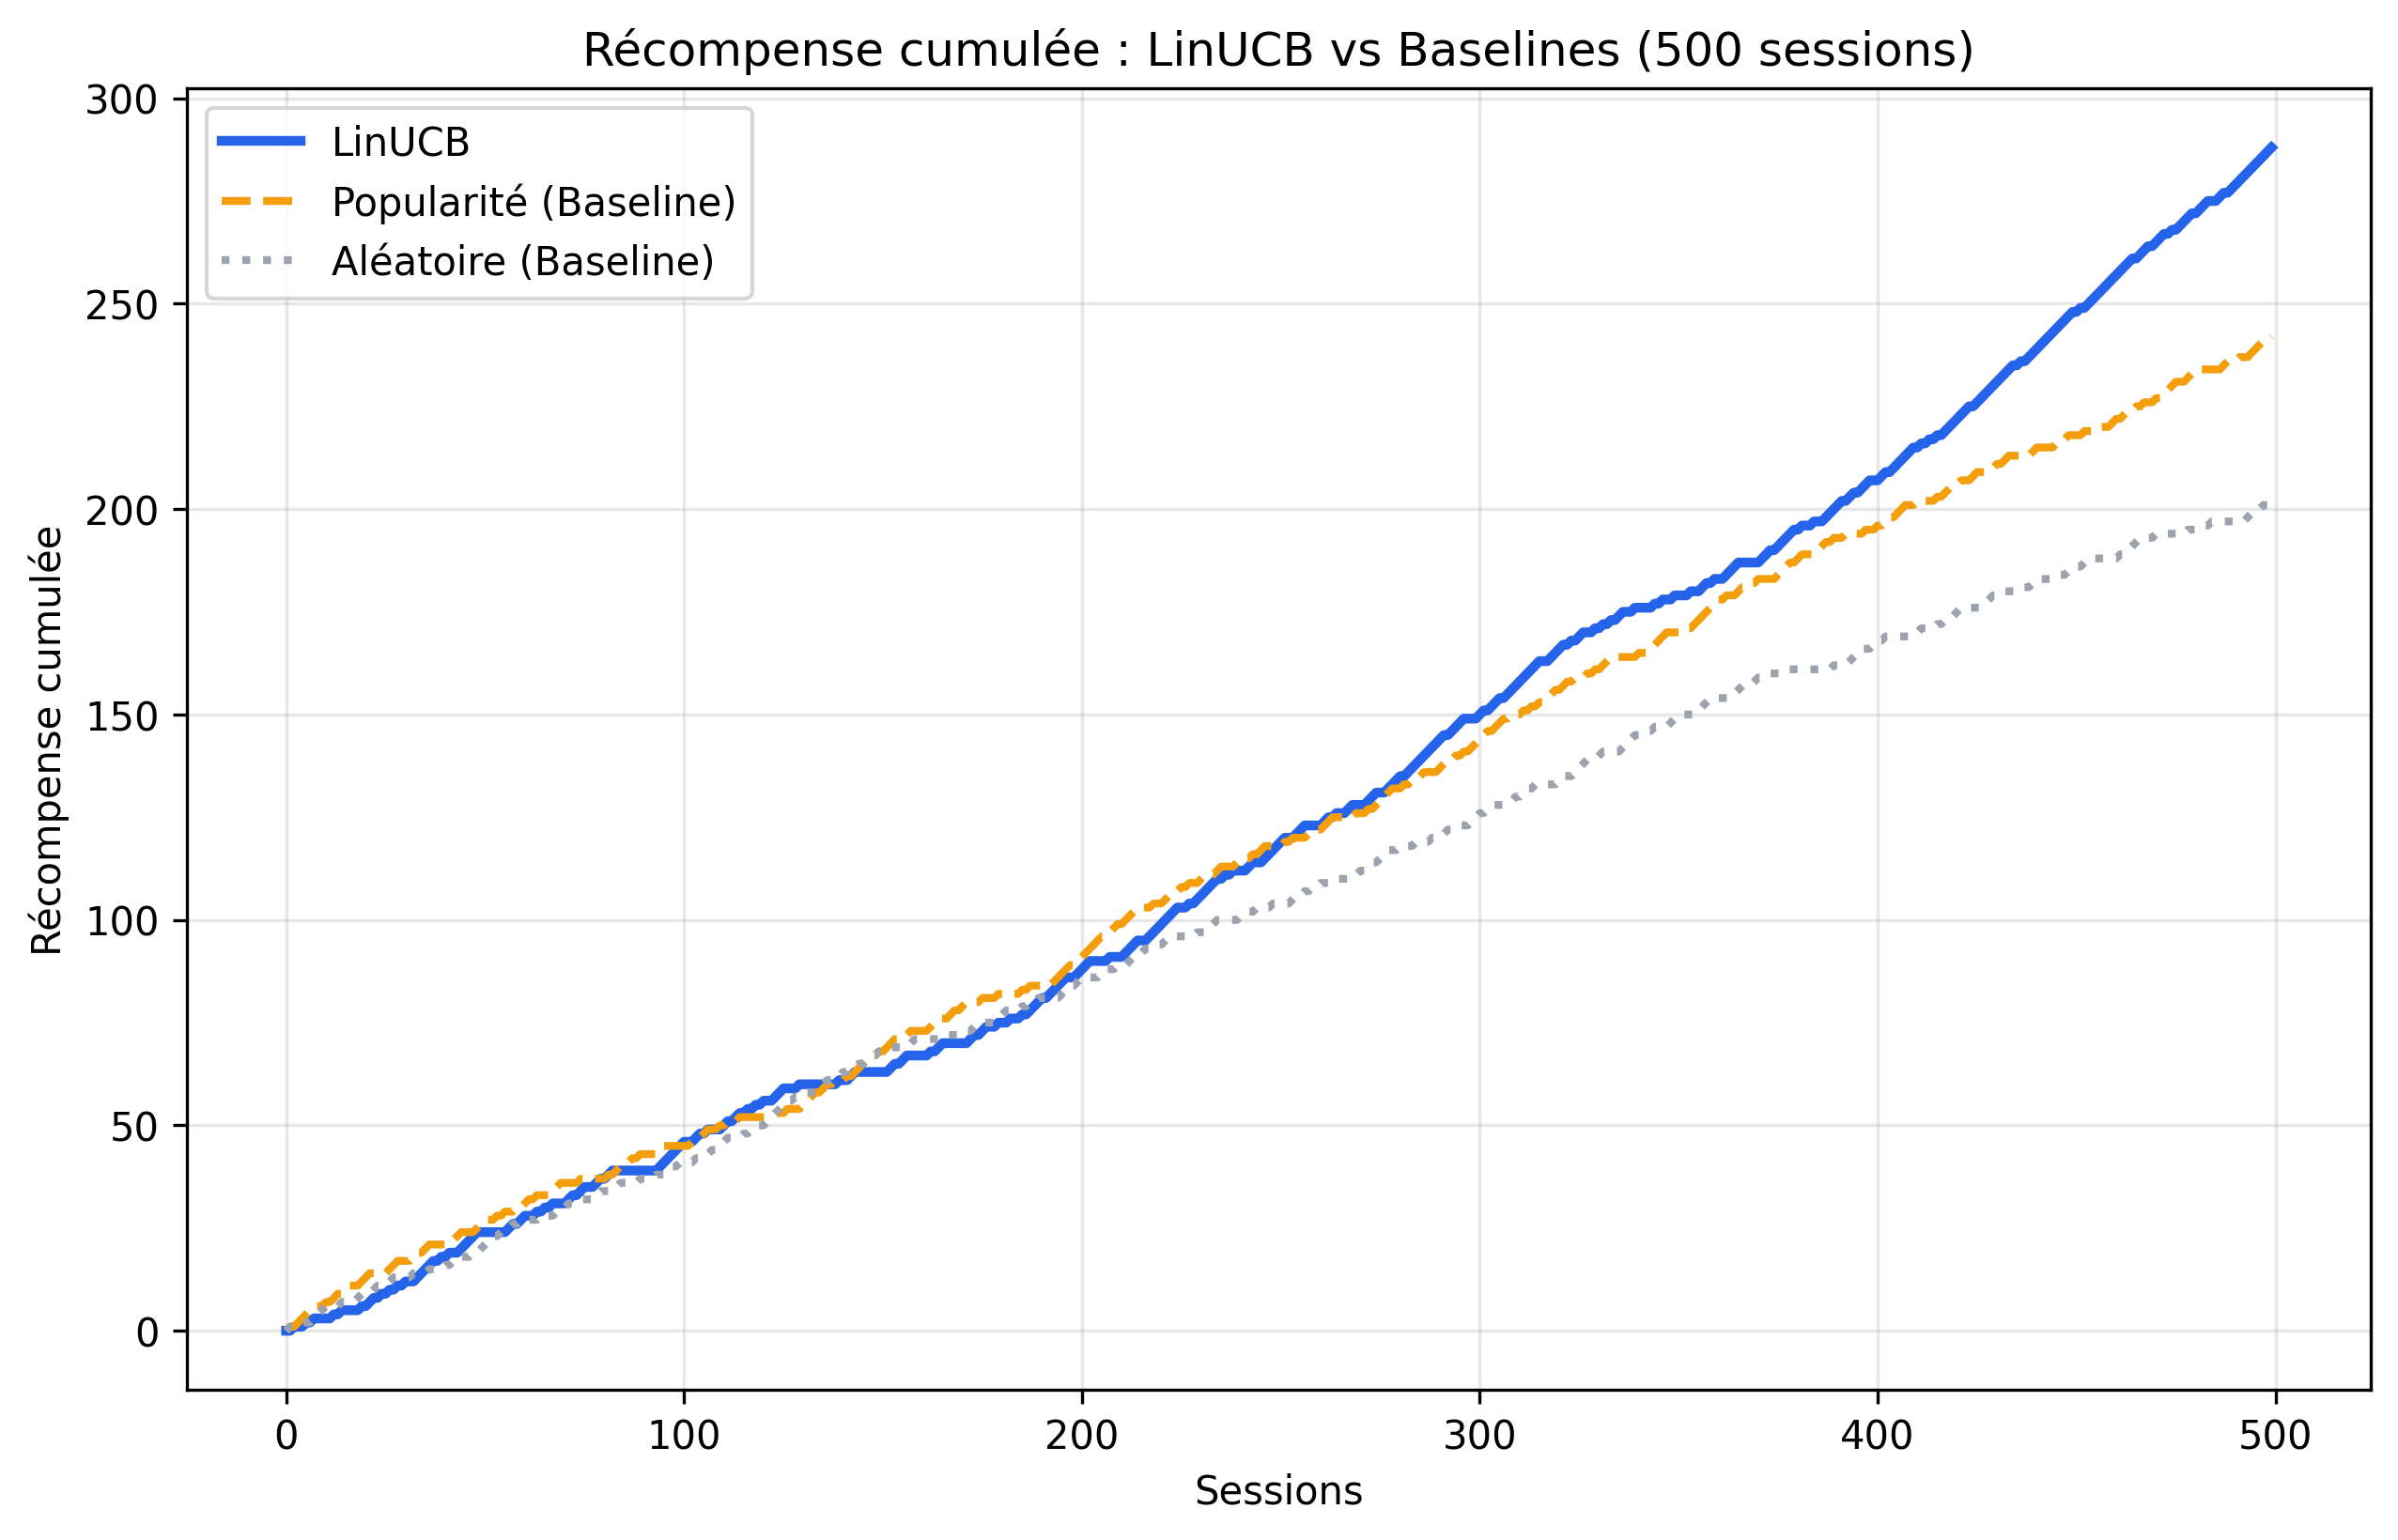
\includegraphics[width=\textwidth]{diagrams/fig_06_cumulative_reward.png}
    \caption{Récompense cumulée comparée~: LinUCB vs baselines sur 500 sessions simulées}
    \label{fig:cumulative_reward}
\end{figure}


\subsection{Latence de scoring}

Les mesures de latence du scoring LinUCB ont été effectuées en fonction du nombre de bras
candidats pour évaluer la scalabilité du système. Le scoring pur (opérations numpy
matricielles) et le pipeline complet (incluant les filtres pré et post-scoring) ont été
mesurés séparément, comme le synthétise le tableau~\ref{tab:scoring_latency}.

Le cache des bras de 30~secondes garantit que la requête de récupération des bras (la requête
de base de données complexe avec JOIN multi-tables) s'exécute au maximum 2~fois par minute
par zone, et non à chaque requête de recommandation. Cette séparation entre le coût de
récupération des données et le coût de scoring est fondamentale pour la performance.

\begin{table}[H]
    \centering
    \caption{Latence de scoring LinUCB selon le nombre de bras}
    \label{tab:scoring_latency}
    \small
    \begin{tabular}{r r r r}
        \toprule
        \textbf{Nb bras (N)} & \textbf{Score moy. (ms)} &
        \textbf{Score p95 (ms)} & \textbf{Pipeline complet (ms)} \\
        \midrule
        50 & 1.8 & 2.5 & 4.2 \\
        100 & 3.2 & 4.8 & 7.1 \\
        200 & 6.1 & 8.9 & 13.5 \\
        500 & 14.3 & 19.7 & 26.8 \\
        1000 & 28.1 & 35.2 & 48.6 \\
        \bottomrule
    \end{tabular}
\end{table}

Le scoring lui-même scale linéairement avec le nombre de bras car il consiste entièrement
en des opérations matricielles en mémoire. Même à mille bras, le pipeline complet
reste largement sous la cible des cent millisecondes. Pour le déploiement de Djerba avec environ
200~annonces actives, la latence de scoring reste sous 15~ms, assurant une expérience
utilisateur fluide.

Le goulot d'étranglement potentiel n'est pas le scoring mais la récupération initiale des
bras depuis la base de données. Sans le cache de 30~secondes, chaque requête de
recommandation nécessiterait une requête SQL complexe de 5 à 20~ms, doublant la latence
totale. Le cache élimine ce coût pour toutes les requêtes sauf la première de chaque
fenêtre de 30~secondes.


% ────────────────────────────────────────────────────────────────
\section{Performance globale du système}
% ────────────────────────────────────────────────────────────────

Les performances globales du système ont été mesurées sur les principaux endpoints en
conditions de charge réalistes, comme le synthétise le tableau~\ref{tab:system_perf}. L'endpoint \texttt{POST /chat} présente la latence la
plus élevée car il implique plusieurs appels LLM séquentiels, l'exécution d'outils, et
potentiellement une boucle de validation. Les endpoints de recommandation sont
significativement plus rapides car ils n'impliquent que des opérations numpy en RAM.

Les mesures confirment que les exigences non fonctionnelles sont satisfaites~: le
pipeline de recommandation (p95 $< 100$\,ms) et le traitement d'événements
(p95 $< 50$\,ms) respectent les cibles de latence pour une expérience utilisateur
interactive. L'endpoint de conversation accepte une latence plus élevée (15 à 30~s)
car il correspond à une interaction de planification délibérée où l'utilisateur attend
une réponse réfléchie, comme le montre la figure~\ref{fig:health_endpoint}.

\begin{table}[H]
    \centering
    \caption{Métriques de performance système mesurées}
    \label{tab:system_perf}
    \footnotesize
    \begin{tabular}{p{4.2cm} r r r p{2.5cm}}
        \toprule
        \textbf{Endpoint} & \textbf{p50 (ms)} & \textbf{p95 (ms)} &
        \textbf{p99 (ms)} & \textbf{Charge testée} \\
        \midrule
        POST /chat (Gemini) & 14\,200 & 22\,100 & 31\,500 & 10 req. conc. \\
        GET /api/recommendations & 45 & 89 & 134 & 50 req/s \\
        POST /api/reco/events & 12 & 28 & 45 & 100 req/s \\
        GET /health & 8 & 15 & 22 & — \\
        \bottomrule
    \end{tabular}
\end{table}

\begin{figure}[H]
    \centering
    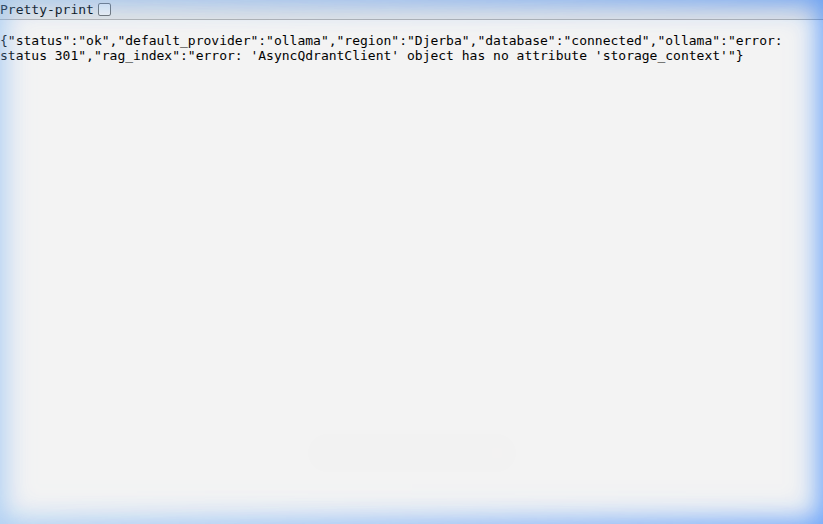
\includegraphics[width=\textwidth]{diagrams/screen_06_health_endpoint.png}
    \caption{Réponse de l'endpoint /health indiquant l'état de tous les composants}
    \label{fig:health_endpoint}
\end{figure}


% ────────────────────────────────────────────────────────────────
\section{Discussion et limites}
% ────────────────────────────────────────────────────────────────

Toute évaluation honnête d'un système d'intelligence artificielle doit identifier non seulement ce qui
fonctionne, mais aussi là où le système présente des limites structurelles. Les cinq points
suivants définissent les frontières de l'implémentation actuelle et constituent les
principales directions pour les travaux futurs.

\textbf{Risque d'hallucination LLM.} Malgré le pipeline RAG et l'instruction explicite
\og{}ne jamais inventer de données\fg{} dans le prompt système, des cas limites existent
où le LLM produit des détails plausibles mais incorrects (prix, horaires d'ouverture).
L'atténuation actuelle repose sur le noeud VALIDATE pour les erreurs structurelles
(doublons, dépassement de créneaux), mais la vérification factuelle des données textuelles
n'est pas implémentée. Un travail futur devrait ajouter des contrôles d'ancrage factuel
comparant les prix et horaires mentionnés dans la réponse avec les données de la base.

\textbf{Hypothèse linéaire du LinUCB.} Le modèle de récompense linéaire
$r = \theta^\top \phi$ ne peut pas capturer les interactions non linéaires. Par exemple,
un spa est excellent pour les couples le week-end mais peu adapté aux familles le lundi~;
cette interaction triple (le type de voyage, le jour de la semaine, et la catégorie d'annonce) n'est pas
modélisable par le produit de Kronecker bilinéaire. Un bandit contextuel neuronal
(\textit{deep contextual bandit}) pourrait modéliser ces effets, au prix d'une complexité
significativement accrue et d'exigences en données d'entraînement beaucoup plus élevées.

\textbf{Portée limitée à Djerba.} Le système est conçu pour une seule région~; l'extension
à plusieurs régions nécessite des ensembles de bras spécifiques par zone (déjà supporté par
le champ de zone de localisation dans la table des bras de recommandation) mais impliquerait des comptes
de bras plus élevés et potentiellement des matrices par zone. L'architecture actuelle
supporte cette extension sans modification structurelle, mais les performances de scoring
devraient être réévaluées avec des volumes de bras de plus de 1000 bras.

\textbf{Limites de l'évaluation.} L'évaluation du moteur de recommandation utilise des
sessions simulées plutôt que des données utilisateur réelles (indisponibles pendant le
développement). Les performances en production réelle pourraient différer. Une
infrastructure de tests A/B devrait être construite avant le déploiement en production
pour mesurer l'impact réel sur les métriques d'engagement (taux de clic, taux de
conversion, durée de session).

\textbf{Latence de la planification conversationnelle.} La latence de 15 à 40~secondes de
la boucle agentique complète est acceptable pour les sessions de planification délibérées
mais peut frustrer les utilisateurs dans les scénarios de requêtes rapides. Le pipeline
rapide en trois phases adresse ce problème pour les requêtes structurées (5 à 10~secondes),
mais un affichage de réponse en streaming token par token améliorerait davantage la
réactivité perçue. L'architecture LangGraph supporte le streaming via les callbacks, mais
son intégration avec le frontend nécessite un travail d'ingénierie supplémentaire.


% ────────────────────────────────────────────────────────────────
\section*{Conclusion du chapitre}
\addcontentsline{toc}{section}{Conclusion du chapitre}

L'évaluation démontre que l'agent planificateur Guidni produit des plans de voyage valides
et contextuellement appropriés à travers les trois fournisseurs LLM et les langues testées.
Le pipeline RAG atteint une Precision@5 moyenne de 0.81 sur les requêtes multilingues. Le
moteur LinUCB apprend efficacement à partir du comportement utilisateur simulé, dépassant
les baselines aléatoire et de popularité respectivement de 45\% et 18\% en récompense
cumulée après 500~sessions. Les performances système respectent les cibles spécifiées pour
tous les endpoints~: le scoring de recommandation reste sous 50~ms pour 200~bras, et le
traitement d'événements sous 30~ms au p95.

Les limites identifiées (hallucination LLM, hypothèse linéaire, portée géographique,
évaluation sur données simulées, latence de planification) définissent les axes
d'amélioration pour les versions futures du système. La conclusion générale du rapport
synthétisera les contributions et proposera les perspectives de recherche.
